\documentclass{standalone}
\usepackage{tikz}
\begin{document}
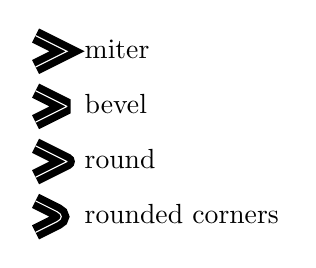
\begin{tikzpicture}
\tikzset{custom/.style={
    black,line width=2mm, postaction={draw=white,thin}}
}

\foreach[count=\y] \join in {miter,bevel,round}{
    \draw[custom,line join=\join]
        (0,2.1-.7*\y)--++(.4,.2)--++(-.4,.2);
    \node[right] at (.5,2.1-.7*\y+.23) {\join};
}

\draw[custom,rounded corners](0,-.7)--++(.4,.2)--++(-.4,.2);
\node[right] at (.5,-.7+.23) {rounded corners};

% {rounded corners=10mm}

\end{tikzpicture}
\end{document}
